 \documentclass[a4paper,12pt,oneside,titlepage]{article} 
\usepackage[T1]{fontenc}
\usepackage[english]{babel}
\usepackage[utf8]{inputenc}
\usepackage{amsfonts} 
\usepackage{amssymb}
\usepackage{amsthm}
\usepackage{amsmath}
\usepackage{graphicx}
\usepackage{array}
\usepackage{booktabs}
\usepackage{siunitx}
\sisetup{output-decimal-marker={.}}
\usepackage{bm}
\usepackage{mathrsfs}
\usepackage[numbers]{natbib}
\usepackage{epstopdf}
\usepackage{subfig}
%\usepackage{subfloat}
\usepackage{multirow}
\usepackage{bm}
\usepackage{float}

\usepackage{verbatim}
\usepackage{hyperref}
\hypersetup{
	colorlinks=true,
	linkcolor=black,
	filecolor=magenta,      
	urlcolor=black,
}
\usepackage{caption}
\graphicspath{{images/}}						%path image
\captionsetup{tableposition=top,figureposition=bottom,format=hang, font=scriptsize}
\usepackage[skip=2pt]{caption}
\usepackage{cleveref}


%\captionsetup{format=myformat}

%\documentclass[paper=a4]{scrartcl}
\usepackage[utf8]{inputenc}
\usepackage[T1]{fontenc}
\usepackage[section]{placeins}
%\usepackage[showframe]{geometry}
%\usepackage{layout}
\setlength{\voffset}{0in}
%\setlength{\headsep}{5pt}
%\textwidth{600}
%\usepackage[a4paper]{geometry}
\usepackage{calc}
\usepackage[textheight=50\baselineskip+10pt]{geometry}

\begin{document}
	
	\thispagestyle{empty}
	\setcounter{page}{0}
	
	\begin{center}
		\huge
		POLITECNICO DI TORINO\\[1.cm]
		\Large
		ICT for Health \\
		\vspace{0.5cm}
		\Large
		Report Laboratory 3\\[1.3cm]
		
		\vspace{0.5cm}
		
\includegraphics[scale=2]{logo.jpg}
	\end{center}
	\vspace{1.cm}
	
	\begin{flushleft}
		\Large
		\noindent {\bfseries Professor:}\\
		Monica Visintin\\[0.2cm]
	\end{flushleft}
	\vspace{1cm}
	
	
	\begin{flushright} 
		\Large
		\noindent{\textbf{Student}:}\\
		Iman Ebrahimi Mehr S250190\\[0.2cm]
	\end{flushright} 
	\vspace{2cm}
	\begin{center}
		\Large
		A.Y.2019-2020
	\end{center}
	
	\newpage
	\thispagestyle{empty}
	\tableofcontents

	
	\newpage
	\section{Introduction}
	Chronic Kidney Disease (CKD) affects about 10\% of the adult population and a lot of them die because of complication related to this illness. The reason why CKD could be ‘fatal’ is that kidney is fundamental for regulation of water in the body, filtering the blood and producing hormones. Today, CKD is still not curable and it can cause people to need care for the rest of their life. In fact, many patients having significant residual kidney function have to start dialysis to preserve this residual kidney function.
	The problem is that treatments like dialysis and kidney transplantation are very expensive; One way to predict Chronic Kidney Disease is using machine learning techniques, for example, the idea behind this project is to build a decision tree1 based on some features of the patient to predict if he is affected or not by CKD. Some of the features considered are taken from blood and urine analysis (for instance, the level of serum creatinine which indicates how the kidney is working or the presence of albumin in the urine that refers to abnormal levels of protein in your body) and some other information are age, obesity, appetite etc..
	To summarize, using a decision tree we can classify a patient, where the possible classes are "affected by CKD" (identified by ‘ckd’ in the dataset) or "not affected by CKD" (identified by ‘notckd’ in the dataset), using as discriminant of our classification some medical features of the patient.
	
	
	\section{Decision tree building}
	\subsection{Reading the dataset}
	The dataset which we used, it was created by L.Jerlin Rubini, Research Scholar of the Alagappa University (\href{https://archive.ics.uci.edu/ml/datasets/chronic_kidney_disease}{\textbf{\underline{source}}}).
	The dataset contains 25 different attributes (numerical and nominal) for each patient (400). The 25th is the given class that tells whereas the patient is ill or not.
	In fact, in this dataset there are some errors due to a wrong notation which don’t allows our program to read it correctly. For this reason, first of all, the dataset has been prepared and fixed: for many patients some parameters were missing and so they were regressed from the features. The regression algorithm used is Ridge Regression with Lagrangian multiplier (tuning coefficient) $\lambda$ equal to 10. Patients with more than 5 missing attributes were discarded, otherwise regression would have been too much approximative; so in the end 337 samples out of 400 were considered.
	Nominal parameters, those with value "good", "poor", "normal", "abnormal", "ckd", "notckd", "yes", "no", "present, "notpresent" have been replaced with 0 or 1 in order to perform the algorithm.
	
	\subsection{Algorithm}
	The used algorithm in this laboratory for the generation of the decision tree is called C4.5 and is already implemented in the library of Python Scikit Learn which module includes decision tree based models for classification and regression. This algorithm, proposed in 1994 by Ross Quinlan, allows to organize a decision tree for classification based on the concept of \textbf{entropy} and \textbf{mutual information}. Entropy is a mathematical concept representing the \textbf{average quantity of information necessary to know which is the value of a certain event}; in other words, it gives a measure of how much the value of a certain event can be predicted.\\
	Mutual information instead represents the reduction of uncertainty of predicting an event given a known feature of that event.\\
	Note that to generation a decision tree, it is required that all features are nominal/categorical, which can take on one of a limited and usually fixed number of possible values. Instead, a numerical features can take on one of an infinite set of possible values (such as a real number). For this reason all numerical features should be transformed in categorical but all features are numerical, so because of this reason we replaced categorical feature with a 0/1 information. This replacement was needed also to apply the regression algorithm.
	
	
	\subsection{Results}
	To read the resulting tree, we have to know that: the label ‘value’ in each box is telling us how many samples at that node fall into each final class, in order (‘notckd’ and ‘ckd’); the label ‘value’ in each box is the number of samples that arrive in that box. Moreover all the features we are considering are treated with the same importance. For this reason, as we can see from the resulting decision tree in figure \ref{albero}, the ‘hemoglobin’ parameter is here considered as 'strongly decisive' even though in reality it is not so. This is due also to the small number of patients we are considering. In fact, reading only the final tree, we could think that all persons with a certain value of hemoglobin are certainly ill. This is true only in the dataset we are considering and not in the real world.
	\begin{figure}[ht]
		\centering
		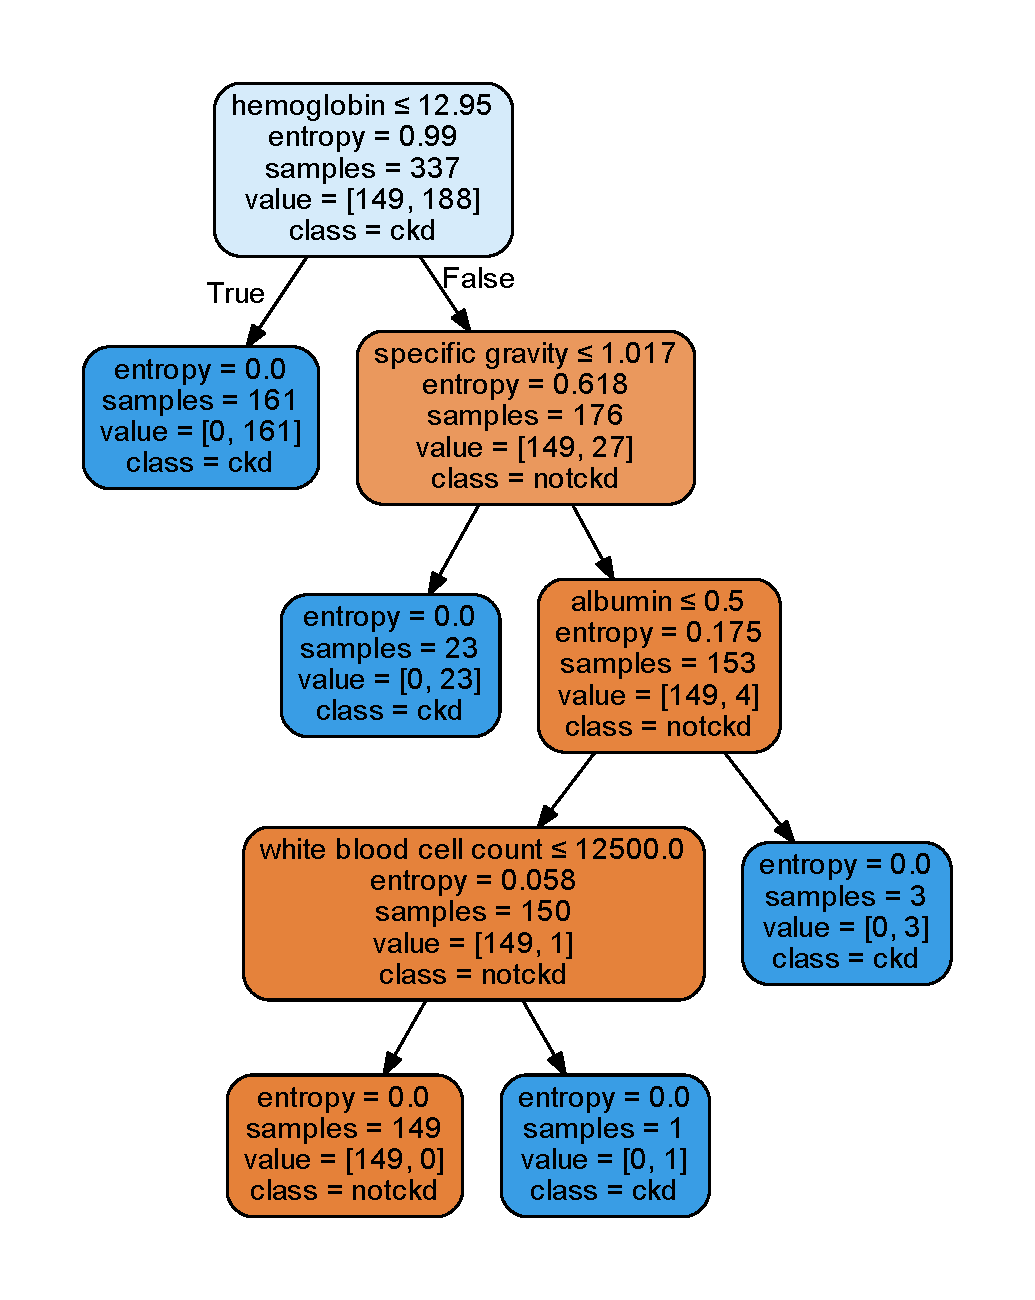
\includegraphics[scale=0.55]{tree.pdf}
		
		\caption{ Decision tree}
		\label{albero}
	\end{figure}
	
	\section{Conclusions}
	As it can be seen from the decision tree, there is a perfect reconstruction of the final class ‘ckd’ or ‘not ckd’. This means, primarily, that the applied regression is correct and so that the predicted value we is correct in order to predict the illness or not of the patient. 
	Having a small dataset is a good thing in order to have a minor computational effort but it is not good for the classification point of view. In fact, having a small dataset can raise some errors, as the one already mentioned for the ‘hemoglobin’. In fact, as in this case, all people with age less than 12 years are affected by CKD. This is true only in the considered dataset (persons with such age are analyzed because is already known they are ill)  but it’s not true in the real world. This happens because this dataset is not representative of the reality. This can lead to some wrong future classifications, in fact could be predicted, looking at the final tree we have produced, that anyone with a given value of hemoglobin is affected by Chronic Kidney Disease and this is simply not true.
	
	
	
	
\end{document}